\documentclass{standalone}
\usepackage{tikz}
\usepackage{ctex,siunitx}
\setCJKmainfont{Noto Serif CJK SC}
\usepackage{tkz-euclide}
\usepackage{amsmath}
\usetikzlibrary{patterns, calc}
\usetikzlibrary {decorations.pathmorphing, decorations.pathreplacing, decorations.shapes,}

\begin{document}
\small
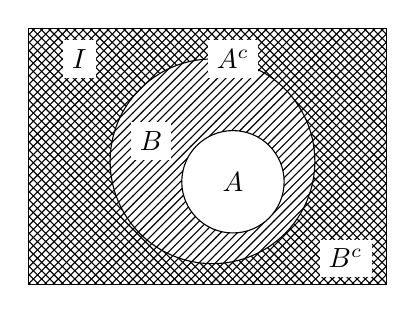
\begin{tikzpicture}[>=stealth,scale=1.3]
  \tkzSetUpPoint[fill=black]
  % \useasboundingbox(-1,-0.75)rectangle(3.7,1.4);
  \fill[pattern=crosshatch, draw](0,0) rectangle (3.5,2.5);
  \fill [white](1.8,1.2) circle (1);
  \draw [pattern=north east lines](1.8,1.2) circle (1);
  \draw [fill=white](2,1)node{$A$} circle (.5);
  \node at (3.1,.25)[fill=white]{$B^c$};
  \node at (.5,2.2)[fill=white]{$I$};
  \node at (1.2,1.4)[fill=white]{$B$};
  \node at (2,2.2)[fill=white]{$A^c$};
\end{tikzpicture}
\end{document}